\chapter{Taratura dei parametri delle leggi di controllo}
\label{cha:1}
Il fulcro centrale della tesi è stato l'implementazione in MATLAB dell'algoritmo di ottimizzazione e il successivo confronto dei diversi risultati ottenuti.\\
La taratura dei parametri è stata fatta tramite l'algoritmo di ottimizzazione Bayesiana, che in \nobreakdash MATLAB si traduce nell'utilizzo della funzione \cite{bayesopt}.

\section{Cenni teorici sull'ottimizzazione bayesiana}
L'ottimizzazione Bayesiana è un algoritmo molto versatile, progettato per ottimizzare modelli a scatola nera, ovvero sistemi dove l'espressione analitica della funzione obiettivo è sconosciuta, così come le sue derivate.\\
L'obiettivo della BO è la risoluzione del problema di ottimizzazione $\underset{\theta}{min} \ J(\theta)$, ovvero trovare per quali valori di $\theta$ la funzione $J(\theta)$ è minimizzata. Il termine $\theta$ può essere rappresentativo di uno o anche più parametri, il cui valore è sconosciuto, ma dove è possibile raccogliere un insieme di misure $J(\theta_1), J(\theta_2), J(\theta_3), \dots, J(\theta_N)$. Inizialmente l'algoritmo genera la funzione obiettivo in modo casuale, la quale viene aggiornata dopo ogni iterazione, a seguito del calcolo di nuovi valori di $J(\theta)$. Questo tipo di approccio statistico fornisce la distribuzione di probabilità di $J(\theta)$ per ogni parametro $\theta$ e questa probabilità è usata per definire una funzione di acquisizione $A(\theta)$. Infatti, la scelta del nuovo parametro da provare per il calcolo dei successivi campioni $J(\theta)$ non è casuale, bensì corrisponde al valore per cui $A(\theta)$ è massimizzata (\figurename \ \ref{fig:BO}). La funzione di acquisizione può essere di diversi tipi, la più comune e anche quella utilizzata in questo lavoro nella \cite{bayesopt} di MATLAB, è la cosiddetta \textit{Expected Improvement (EI)}.\\
\begin{figure}[htb]
	\centering
	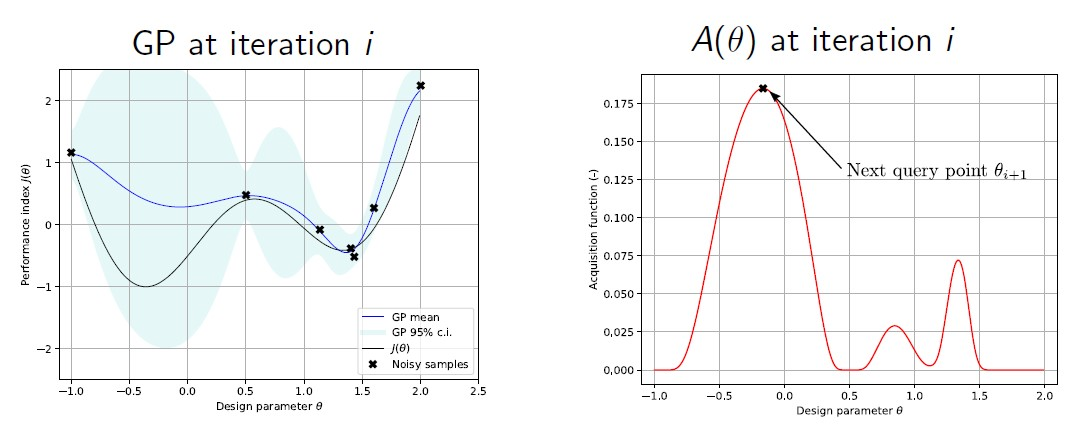
\includegraphics[scale=0.6]{figure/BO.jpg}
	\caption{Esempio di ottimizzazione bayesiana con modello surrogato e funzione di acquisizione}
	\label{fig:BO}
\end{figure}

Sebbene ci siano anche altri algoritmi che seguono principi simili, l'innovazione dell'ottimizzazione bayesiana sta proprio nel modo in cui il successivo punto di campionamento viene scelto e nel suo tentativo di convergere all'ottimo globale nel minor numero di iterazioni.\\
Grazie all'implementazione in MATLAB di questo tipo di ottimizzazione è stato possibile realizzare la taratura dei parametri per le due strategie di controllo, per le quali la cifra di costo che si vuole minimizzare è rappresentata dal valore efficacie dell'accelerazione verticale del veicolo. 

\section{Implementazione di \textit{bayesopt}}
La funzione di MATLAB \textit{bayesopt} richiede come input la funzione obiettivo che si vuole minimizzare e i parametri da ottimizzare. La cifra di costo richiesta come input corrisponde al calcolo dell'indice di performance $J$ per ogni simulazione. Nell'inizializzare le variabili da ottimizzare, che sono gli elementi del vettore $\tilde{k}$ e della matrice $P_x$, è necessario specificare il range di valori da esplorare per i diversi parametri, che a priori non è possibile conoscere, ma si può trovare a seguito di alcune simulazioni.\\
Considerando la legge lineare, l'argomento della saturazione in valore assoluto, nell'equazione \eqref{leggelin}, non può superare $\frac{\tilde{f}_{max}}{2}$, altrimenti risulterebbe un calcolo inutile. Sono state quindi fatte diverse simulazioni, con una configurazione passiva della sospensione, variando il valore di $u_{MR}$, in modo da calcolare il quantile al 95\% per ogni variabile di stato e poter poi trovare il range possibile per ogni parametro:
\begin{equation}
	\centering
	sat_{\frac{\tilde{f}_{max}}{2}}(\tilde{k}x) \  \Longrightarrow \  k_{i-max}*x_{i-max} = \frac{f_{max}}{2} \  \Longrightarrow \  k_{i-max} = \frac{f_{max}}{2}*\frac{1}{x_{i-max}}.
	\label{rangeparametri}
\end{equation}
In modo analogo sono stati i svolti i calcoli per trovare il range per i parametri della matrice $P_x$ della legge di controllo quadratica.\\

In MATLAB il codice necessario per implementare l'algoritmo di ottimizzazione risulta essere il seguente:
\begin{figure}[htb]
	\centering
	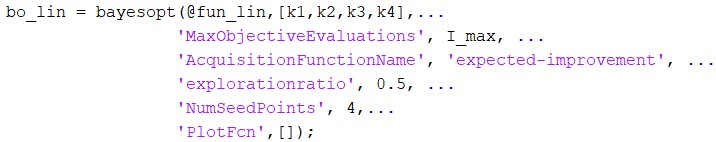
\includegraphics[scale=0.7]{figure/BOlin.jpg}
	\caption{Implementazione in MATLAB della funzione \textit{bayesopt}}
	\label{fig:bayesopt}
\end{figure}

\section{Analisi dei risultati}
Le simulazioni sono state fatte tutte con le impostazioni della \cite{bayesopt} mostrate in \figurename \ \ref{fig:bayesopt}. \textit{AquisitionFunctionName} indica il tipo di funzione di acquisizione utilizzata nell'algoritmo di ottimizzazione, l'\textit{explorationratio} fa riferimento alla propensione dell'algoritmo ad esplorare nuovi punti da campionare, più basso è, più si evita di "sprecare" iterazioni in punti non importanti, ma si rischia di rimanere bloccati in minimi locali. Infine, \nobreakdash\textit{NumSeedPoints} esplicita il numero di volte per cui si calcola la funzione di costo con parametri presi in modo casuale, nel range possibile indicato.\\
Sul grafico in \figurename \ \ref{fig:plotJ} è mostrato l'andamento della minimizzazione della funzione obiettivo $J$ in relazione al numero delle iterazioni.
\begin{figure}[htb]
	\centering
	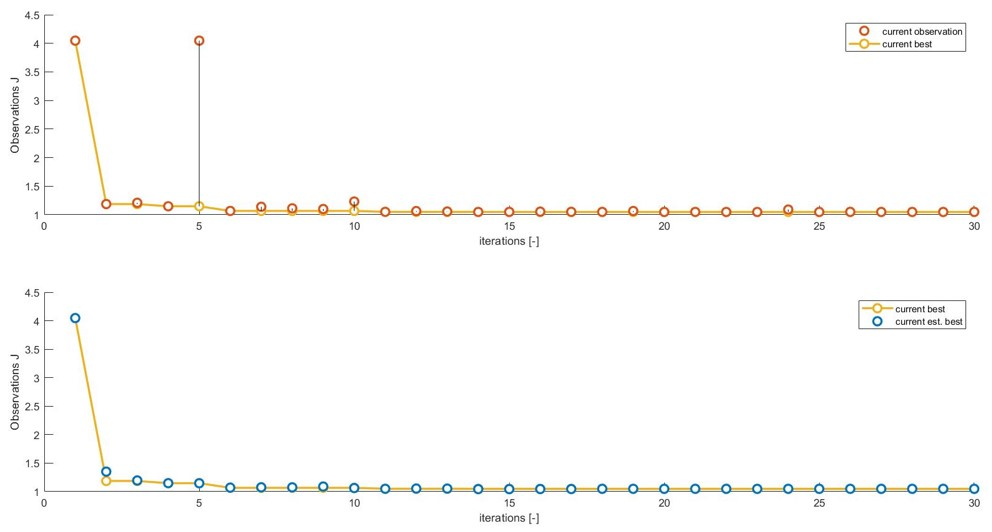
\includegraphics[scale=0.7]{figure/plotJ.jpg}
	\caption{Implementazione in MATLAB della funzione \textit{bayesopt}}
	\label{fig:plotJ}
\end{figure}\\
Per un'ottimizzazione più completa possibile, le simulazioni sono state eseguite con un numero di iterazioni sufficientemente elevato e per più volte tramite ciclo \textit{for}, in modo da osservare anche la variabilità dei risultati con un diverso ingresso $z_r$.\\

\subsection{Legge di controllo lineare}
\label{lin}
In \tablename \ \ref{risultatileggelin} è mostrato il resoconto di 10 diversi processi di ottimizzazione, per ognuno dei quali è stato generato un diverso input $z_r$. La tabella sottolinea come, in ogni simulazione, l'implementazione della legge di controllo lineare per la sospensione semi-attiva, faccia sì che l'indice di performance sia minore rispetto ad una configurazione passiva della sospensione. Questa è una prima dimostrazione di come una legge di controllo lineare vada a migliorare le prestazioni di comfort, rispetto ad una configurazione passiva della sospensione.\\
\'E possibile inoltre osservare, come i parametri $k_1, k_3$ e $k_4$, al variare delle simulazioni, abbiano rispettivamente dei valori molto simili, mentre il  parametro $k_2$ assuma  sempre dei valori molto differenti nelle diverse ottimizzazioni. Il fatto che $k_2$ vari molto indica che questo parametro, associato alla variabile di stato $z_s$ non è così fondamentale per la legge di controllo. Questa osservazione conferma ciò che potrebbe essere intuibile già "ad occhio nudo", ovvero che la posizione della macchina non ha nessuna influenza sul sistema e sulle sospensioni.\\
Questo risultato si è rivelato molto importante per il prosieguo del lavoro, infatti per le successive simulazioni, nella taratura dei parametri tramite ottimizzatore, è stato omesso il parametro $k_2$, semplificando quindi il problema e risparmiando tempo.\\
\renewcommand\arraystretch{1.4} 
\begin{table}[hbt]
	\centering
	\begin{tabular}{|c||c|c|c|c||c|c|}
		\hline
		$\# iterazioni$ & \textbf{$k_1$} & \textbf{$k_2$} & \textbf{$k_3$} & \textbf{$k_4$} & \textbf{$J_{ottim} \ [\frac{m}{s^2}]$} & \textbf{$J_{u_{MR} = 0} \ [\frac{m}{s^2}]$}\\
		\hline
		\hline 100 & 4994.7 & 1256.1 & -48964.9 & -57686.1 & 1.0410 & 1.0854\\
		\hline 100 & 4891.1 & 916 & -42489 & -52825 & 1.0600 & 1.1372\\
		\hline 100 & 4882.6 & -1068.2 & -45049.1 & -57644.7 & 1.0519 & 1.1044\\
		\hline 100 & 4832.6 & -1626.5 & -37832.2 & -52204.1 & 1.1003 & 1.1770\\
		\hline 100 & 5112.3 & -184.7 & -46131.6 & -56255.9 & 1.0662 & 1.1053\\
		\hline 100 & 4836.7 & 1862.5 & -39944.8 & -51648.3 & 1.0578 & 1.1528\\
		\hline 100 & 4778.6 & 1070.9 & -48280.1 & -55971.2 & 1.0671 & 1.1114\\
		\hline 100 & 4965.8 & 416.8 & -66707.4 & -58684.9 & 1.0560 & 1.0860\\
		\hline 100 & 4863.3 & -1386.5 & -43122.3 & -56622.4 & 1.0697 & 1.1130\\
		\hline 100 & 5027.5 & -1568.5 & -44443 & -55609.9 & 1.0613 & 1.1144\\		
		\hline
	\end{tabular}
	\caption{Taratura dei parametri per 10 simulazioni, eseguite con un diverso input $z_r$}
	\label{risultatileggelin}
\end{table}\\
L'analisi dei risultati più significativa e immediata risulta essere quella fatta nel dominio della frequenza, tracciando il grafico della funzione di trasferimento del modello implemetato con la legge di controllo e il modello con la configurazione passiva della sospensione. In questo modo è possibile apprezzare meglio la differenza tra i modelli, in termini di prestazioni di comfort (\figurename \ \ref{fig:confronto}).
\begin{figure}[htb]
	\centering
	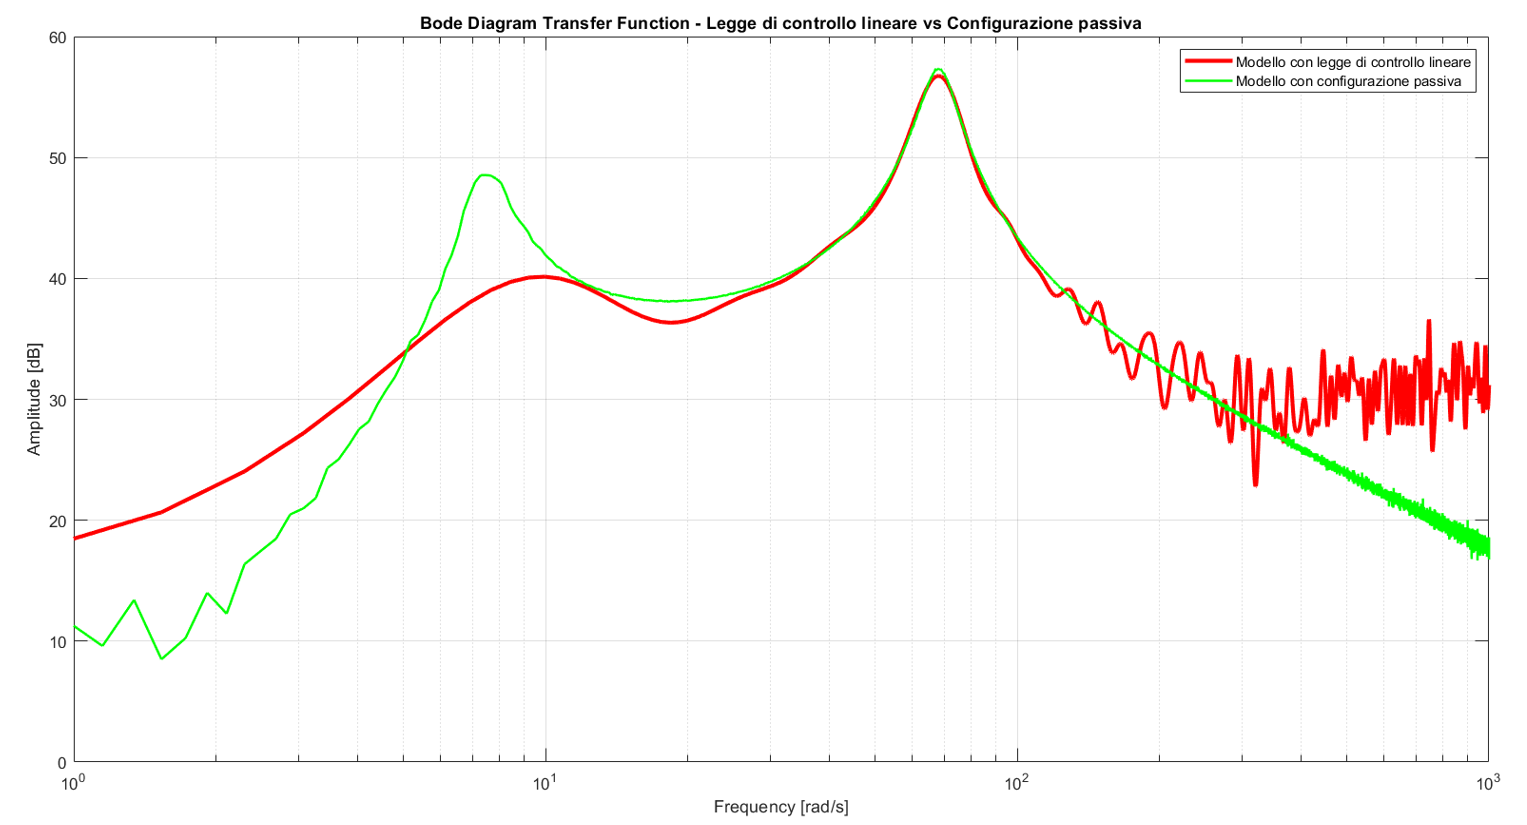
\includegraphics[scale=0.4]{figure/confrontoPas-Lin.png}
	\caption{Diagramma di Bode del modulo della FdT : modello con legge lineare e configurazione passiva}
	\label{fig:confronto}
\end{figure}\\
Dalla \figurename \ \ref{fig:confronto} la differenza tra i vari modelli è rimarcata soprattutto in corrispondenza del primo picco, dove per il modello implementato con la legge di controllo lineare, è decisiamente più smussato.\\
Ad alte frequenze risulta più difficile per la funzione \textit{tfestimate} stimare in modo preciso il modulo della funzione di trasferimento, in quanto ci si sta avvicinando alla frequenza di campionamento utilizzata e per questo sono presenti molte oscillazioni nel grafico.


\subsection{Legge di controllo quadratica}
\label{quad}
In modo analogo a quanto fatto per la legge di controllo lineare, è stata implementata la legge di controllo quadratica \eqref{leggequad}, con ottimizzazione dei parametri della matrice $P_x$. Essendo la matrice simmetrica 4x4 i parametri da ottimizzare sono 10 in tutto, ma avendo analizzato i risultati ottenuti per la legge lineare, si possono porre a zero tutti i termini che includono la variabile di stato $z_s$ e quindi ne consegue che gli elementi da ottimizzare sono: $p_{1,1}$, $p_{1,3}$, $p_{1,4}$, $p_{3,3}$, $p_{3,4}$, $p_{4,4}$.\\
In un primo momento i risultati ottenuti non sono stati così soddisfacenti, infatti, per ogni simulazione, il valore dell'indice di performance per il modello implementato con la legge di controllo quadratica risultava essere sempre maggiore rispetto al modello con configurazione passiva, circa $2.4\frac{m}{s^2}$.\\
A questo punto è stato fondamentale fare un'analisi di sensitività della cifra di costo in funzione delle dimensioni della "scatola", in cui l'ottimizzatore va a ricercare i parametri della legge di controllo. Sono state fatte ulteriori simulazioni aumentando, anche di diversi ordini di grandezza, il range di valori entro il quale l'algoritmo di ottimizzazione prende i parametri. Si è osservato che per tre ordini di grandezza in più rispetto ai valori limite, trovati tramite la formula \eqref{parametri}, il valore della cifra di costo migliora sensibilmente ($1.3\frac{m}{s^2}$), senza però riuscire ad ottenere un valore simile a quello ottenuto con una configurazione passiva.\\

\section{Osservazioni finali}
Tramite il modello controllato attraverso la legge quadratica non si sono raggiunti degli ottimi risultati, per quanto riguarda l'indice di performance, eppure il modulo della funzione di trasferimento ci ha fornito delle importanti informazioni sulle prestazioni di questa strategia di controllo. 
In \figurename \ \ref{fig:confrontolinquad} è possibile osservare la differenza, nel dominio della frequenza, tra il modello con una legge di controllo lineare e quello con legge di controllo quadratica. Se si considera tutto il campo di validità, una strategia di controllo lineare fornisce delle migliori prestazioni, così come indica l'indice $J$. Tuttavia, la legge di controllo quadratica fornisce migliori performance a frequenza basse e quindi presenta comunque una buona soluzione per alcuni casi particolari.\\
\begin{figure}[htb]
	\centering
	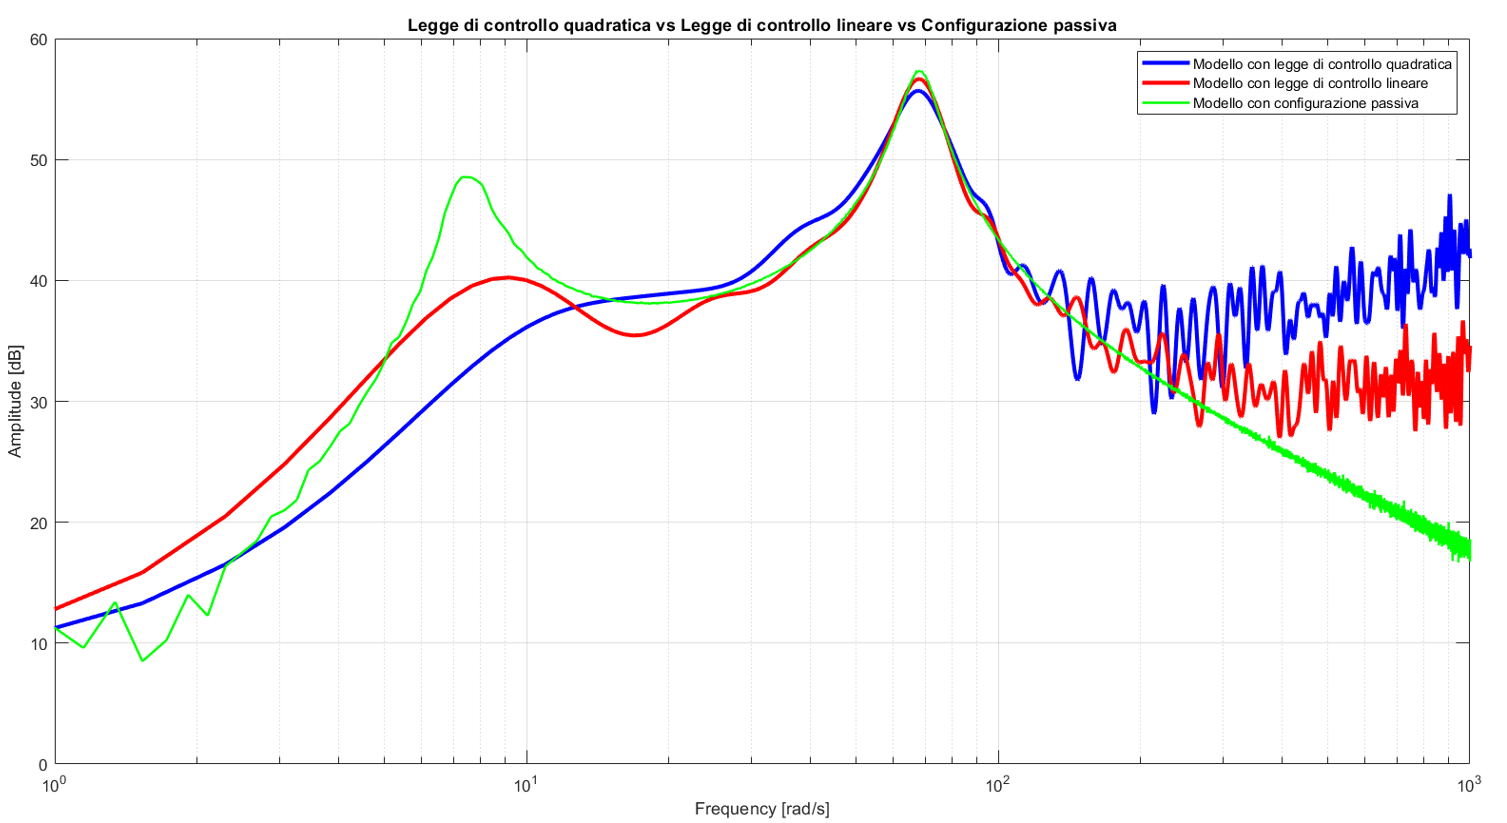
\includegraphics[scale=0.4]{figure/confrontoPas-Lin-Quad.png}
	\caption{Diagramma di Bode del modulo della FdT : modello con legge lineare, legge quadratica e configurazione passiva}
	\label{fig:confrontolinquad}
\end{figure}\\

\newpage
Considerando i risultati ottenuti con le due diverse strategie di controllo presentate pocanzi, si è voluto provare ad adottare una soluzione che combinasse la legge di controllo lineare e quella quadratica. L'obiettivo era quello di ottenere dei risultati che ci fornissero le migliori performance possibili a basse frequenze, come la legge quadratica, ma anche a medio-alte frequenze, secondo l'andamento della legge lineare. In Simulink è stato quindi implementato il modello rappresentativo dell'equazione \eqref{leggelinquad}.\\
Il valore dell'indice di performance ottenuto per questo modello è risultato molto simile a quello della legge lineare, però, come si puù osservare dal grafico in \figurename \ \ref{fig:confrontofinale}, in generale non si vedono miglioramenti importanti nel combinare le due leggi insieme.

\begin{figure}[htb]
	\centering
	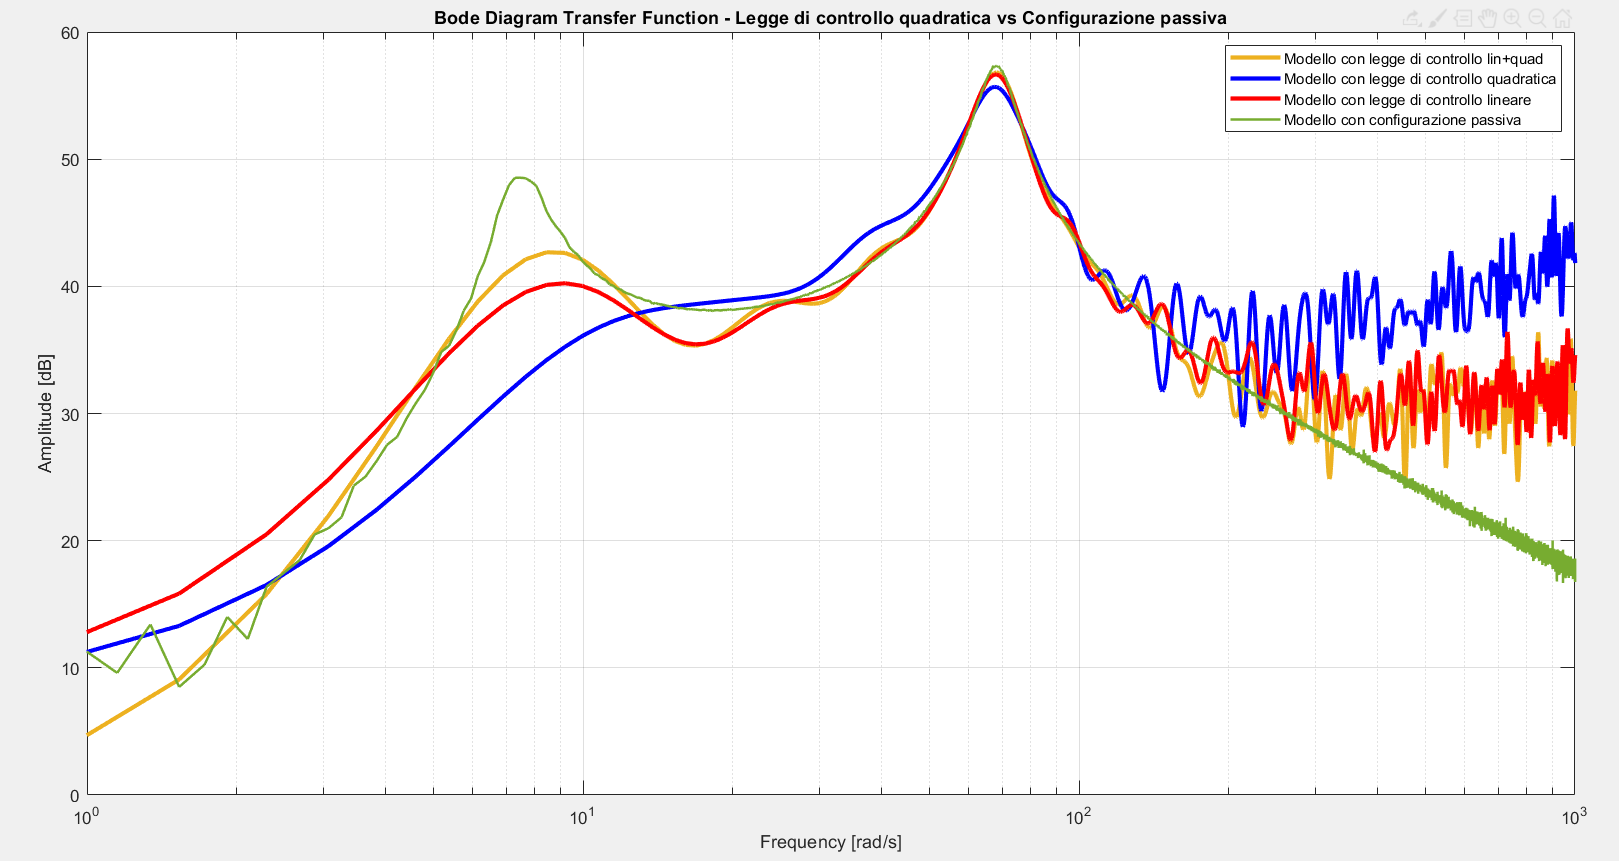
\includegraphics[scale=0.26]{figure/confrontofinale.png}
	\caption{Diagramma di Bode del modulo della FdT : confronto fra tutte le strategie di controllo implementate}
	\label{fig:confrontofinale}
\end{figure}



